\chapter{Remote Work, Collaboration, and the Future Already Underway}

The passage begins with a forecasting question: what are the three biggest technology trends over the next five to ten years? The answer does not give us a neat list. It immediately narrows to one developed cluster of ideas. Some of the future has already arrived, the pandemic accelerated it, remote work is the visible form, and collaboration is the deeper operating category. In these notes we keep that order. We begin with the question, watch it become a diagnosis of the present, and then reconstruct, cautiously and qualitatively, the mechanism that makes that diagnosis persuasive.

\section{A Forecast Recast in the Present Tense}

We first hear a question about the future. The speaker's first move is to refuse a purely speculative answer. Some of what matters has already happened, and the pandemic accelerated it. That is the key pivot of the passage.

A compact way to preserve that claim is
\begin{equation}
A_{\mathrm{remote},\mathrm{now}} > A_{\mathrm{remote},\mathrm{past}} .
\end{equation}
Here \(A_{\mathrm{remote}}\) denotes the effective adoption or practical intensity of remote work. The inequality is qualitative. It does not claim a measured coefficient or a precise time series. It simply records the speaker's order of thought: before we ask what technology will become, we notice what has already crossed into ordinary practice.

This is why the answer feels less like a trend report than like a guided explanation. We are not yet being asked to imagine a distant world. We are being asked to recognize a transition already in motion.

\section{Remote Work First, Collaboration Beneath It}

The first named trend is remote work. But the lecturer does not leave the matter there. He immediately widens the frame: not only remote work, but any type of collaboration. That small broadening does almost all the conceptual work in the excerpt.

Remote work is the visible surface. Collaboration is the underlying category. A team can work remotely only if it can still coordinate, communicate, hand work across boundaries, and maintain shared context. In that sense, the real question is not simply where people work. It is how work remains joined together when distance intervenes.

We therefore distinguish four objects:
\begin{itemize}
\item \(B\): effective internet access speed or bandwidth,
\item \(C\): the capability and maturity of collaboration tools,
\item \(P_{\mathrm{comm}}\): the practical productivity of the communication layer,
\item \(V_{\mathrm{remote}}\): the viability of remote work as a stable operating mode.
\end{itemize}

The transcript does not present these symbols, but they provide a cautious formal skeleton for the speaker's logic. We should also note a structural subtlety. In the spoken order, the pandemic is mentioned before the infrastructure. In the causal order, however, the infrastructure explains why the accelerated adoption could hold.

\section{Why This Became Possible}

The lecture now invites its own natural question. If remote work and distributed collaboration are so central, why were they not central earlier? The answer comes by way of contrast: in the past, we did not have the relevant tools in a form strong enough to support this mode of work.

\subsection{Question \& Answer}

\paragraph{Question.} Why is this way of working viable now when it was not viable before?

\paragraph{Answer.} Because the enabling layer improved. The speaker names two improvements in particular: fast internet access speeds and collaborative tools. Those do not merely ornament work. They change the feasible set of work arrangements.

A cautious reconstruction is to separate the communication layer from the adoption layer. First we model communication productivity as a monotone function of connectivity and tooling:
\begin{align}
P_{\mathrm{comm}} &= g(B,C),\\
\frac{\partial g}{\partial B} &> 0,
\qquad
\frac{\partial g}{\partial C} > 0 .
\end{align}
Next we let remote-work viability depend monotonically on the productivity of that communication layer:
\begin{align}
V_{\mathrm{remote}} &= h(P_{\mathrm{comm}}),\\
\frac{dh}{dP_{\mathrm{comm}}} &> 0 .
\end{align}
Combining the two gives the worked qualitative derivation
\begin{align}
\frac{\partial V_{\mathrm{remote}}}{\partial B}
&=
\frac{dh}{dP_{\mathrm{comm}}}
\frac{\partial g}{\partial B}
>0,\\
\frac{\partial V_{\mathrm{remote}}}{\partial C}
&=
\frac{dh}{dP_{\mathrm{comm}}}
\frac{\partial g}{\partial C}
>0 .
\end{align}
This is not a data-driven theorem extracted from the interview. It is a minimal formalization of the causal logic that the speaker gives in words: faster connectivity and better tools raise communication productivity, and that in turn raises the viability of remote work.

We may now summarize the passage's before-and-after contrast as
\begin{equation}
P_{\mathrm{comm},\mathrm{now}} > P_{\mathrm{comm},\mathrm{past}}
\qquad\Longrightarrow\qquad
V_{\mathrm{remote},\mathrm{now}} > V_{\mathrm{remote},\mathrm{past}} .
\end{equation}
Once that inequality is in place, the opening observation follows naturally:
\begin{equation}
A_{\mathrm{remote},\mathrm{now}} > A_{\mathrm{remote},\mathrm{past}} .
\end{equation}

Because no validated board figure survives from this lecture, the right visual aid here is an editorial schematic of the argument rather than a claimed reconstruction of a lost classroom drawing:

\begin{figure}
\centering
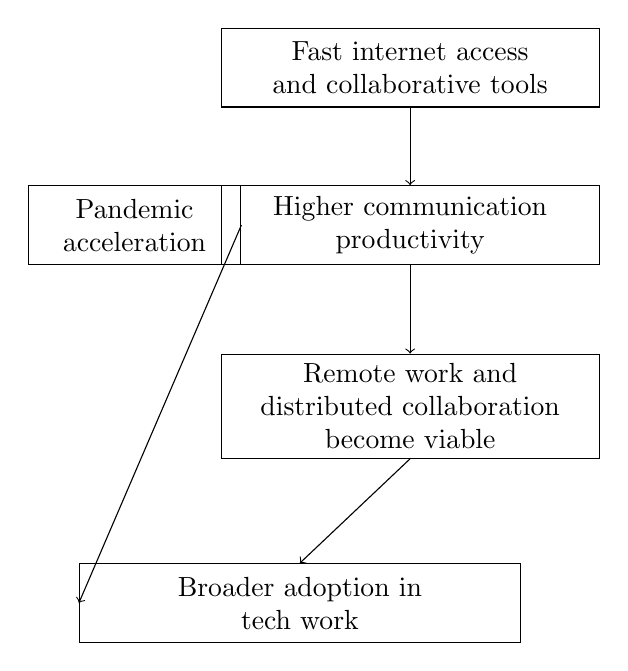
\begin{tikzpicture}[x=1cm,y=1cm]
\node[draw, rectangle, minimum width=2.7cm, minimum height=1.0cm, align=center] (a) at (-2.1,-2.0) {Pandemic\\acceleration};

\node[draw, rectangle, minimum width=4.8cm, minimum height=1.0cm, align=center] (b) at (1.4,0.0) {Fast internet access\\and collaborative tools};
\node[draw, rectangle, minimum width=4.8cm, minimum height=1.0cm, align=center] (c) at (1.4,-2.0) {Higher communication\\productivity};
\node[draw, rectangle, minimum width=4.8cm, minimum height=1.2cm, align=center] (d) at (1.4,-4.3) {Remote work and\\distributed collaboration\\become viable};
\node[draw, rectangle, minimum width=5.6cm, minimum height=1.0cm, align=center] (e) at (0.0,-6.8) {Broader adoption in\\tech work};

\draw[->] (b.south) -- (c.north);
\draw[->] (c.south) -- (d.north);
\draw[->] (d.south) -- (e.north);
\draw[->] (a.east) -- (e.west);
\end{tikzpicture}
\end{figure}

The diagram is deliberately narrow and vertical. It also preserves an important distinction: the pandemic accelerates adoption, but the enabling infrastructure explains why adoption can be sustained rather than merely forced for a moment.

\section{Zoom, Slack, and Even Email}

Only after the general mechanism has been named does the lecture move to specific tools. This order matters. Zoom, Slack, and email are not presented as a random list of fashionable products. They serve as evidence that the communication layer itself has become more productive.

We may collect the examples as
\begin{equation}
\mathcal{T}_{\mathrm{comm}}
=
\{\mathrm{Zoom},\mathrm{Slack},\mathrm{email}\}.
\end{equation}
The set is not a taxonomy of the whole market. It is a compact record of the speaker's move from mechanism to concrete instances.

Three points are worth preserving.

\paragraph{Claim.} These tools are more productive than they used to be.

\paragraph{Mechanism.} Better connectivity and better software reduce the friction of coordination. Communication becomes less intermittent, less fragile, and less costly in attention.

\paragraph{Consequence.} Once that friction falls, remote work is no longer merely an emergency substitute for in-person work. It becomes an ordinary and scalable way of organizing technical labor.

The mention of email is especially revealing. Zoom and Slack obviously belong to the modern collaboration stack. ``Even email'' widens the claim. The speaker is not praising one app category; he is saying that the entire communication environment has become more effective.

\section{The Future of Tech Work}

The closing statement is crisp: collaboration is definitely the future for tech work, and remote work comes with it. We should preserve the asymmetry. The deeper trend is collaboration; remote work is one of its principal social and organizational consequences.

A compact shorthand for the closing hierarchy is
\begin{equation}
C \uparrow
\;\Longrightarrow\;
P_{\mathrm{comm}} \uparrow
\;\Longrightarrow\;
V_{\mathrm{remote}} \uparrow
\;\Longrightarrow\;
A_{\mathrm{remote}} \uparrow .
\end{equation}
Again, we should read this as ordered causal shorthand, not as a calibrated model. It captures the shape of the answer. Better tools raise communication productivity; higher communication productivity makes distributed work viable; viable distributed work raises adoption; and the result is a collaboration-centered form of tech work.

For entrepreneurship, the implication is immediate. A founder should not think only in geographic terms, as if the central question were whether people are in an office or at home. The deeper question is operational: how does the firm coordinate, how does information move, how do tools reduce delay and ambiguity, and how does the business remain coherent when work is distributed across space?

\section{Summary}

The excerpt begins with a question about the next five to ten years, but it develops only one answer cluster in full. Some of the future has already arrived. The pandemic accelerated its adoption. Remote work is the first visible manifestation, but collaboration is the deeper category. Fast internet access and better tools make the communication layer more productive, and that increased productivity makes remote work viable on a larger scale.

That is the order we should keep on the page. We start with a forecast, pivot to an already visible transition, ask why that transition became workable, and end with the speaker's hierarchy: collaboration first, remote work second.